\begin{frame}{Υπερδειγματοληψία πραγματικής σάρωσης σε μη γραμμικές περιοχές \tikzxmark}

  \definecolor{r}{rgb}{1 0 0}
  \definecolor{b}{rgb}{0 0.4470 0.7410}

  \noindent\makebox[\linewidth][c]{%
  \begin{minipage}{\linewidth}
    \begin{minipage}{0.3\linewidth}
      \begin{figure}
        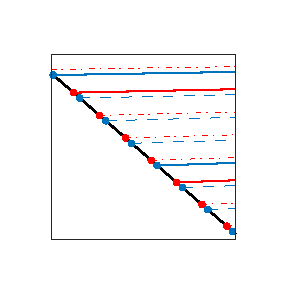
\includegraphics{./figures/slides/ch6/oversampling/false_oversampling_2}
      \end{figure}

      \begin{textblock}{14}(1,4.1)\scriptsize
        \textcolor{b}{$\mathcal{S}_R^{\text{ - -interp}}(\theta)$} \hspace{0.05cm} \textcolor{r}{$\mathcal{S}_V^{\text{ - -interp}}(\hat{\theta})$}
      \end{textblock}
      \begin{textblock}{14}(5.7,4.1)\scriptsize
        \textcolor{b}{$\mathcal{S}_R^{\text{ - -interp}}(\theta)$} \hspace{0.05cm} \textcolor{r}{$\mathcal{S}_V^{\text{ - -interp}}(\hat{\theta})$}
      \end{textblock}
    \end{minipage}
    %\hfill
    \begin{minipage}{0.3\linewidth}
      \begin{figure}
        \animategraphics[autoplay,loop]{1}{./figures/slides/ch6/oversampling/false_oversampling_}{3}{4}
      \end{figure}
    \end{minipage}
    %\hfill
    \begin{minipage}{0.3\linewidth}
      %\begin{figure}
        %\animategraphics[autoplay,loop]{2}{./figures/slides/ch6/oversampling/false_oversampling_}{1}{2}
      %\end{figure}
    \end{minipage}
  \end{minipage}
  }
\end{frame}
